\chapter{Descrição do Sistema ``Admins''}
\label{chap4}

Dado a escolha de um banco de dados em grafo como o Neo4j, o sistema ``Admins'' veio para resolver o problema de ser complicado e pouco seguro gerenciar os dados diretamente através de uma Cypher no banco, sendo facilmente possível realizar consultas muito pesadas, ou que tem consequências difíceis de reverter, de maneira acidental.

Foi então desenvolvido uma interface para usuários interagirem com o banco, podendo criar, editar, conectar e desconectar arbitrariamente nós no banco de dados. Esse sistema foi nomeado de 'admins', graças ao subdomínio utilizado para hospoedá-lo.

\section{Perfis e Listas}

Junto com o time de Design, identificamos uma maneira de entender e visualizar o grafo que está armazenado no banco, dando para cada nó uma página de perfil, que mostra e permite edição de suas propriedades e relações, além de uma página de lista/pesquisa para cada rótulo (relevante) no banco de dados. Endentendo este isomorfismo, conseguimos criar esta interface e permitir os usuários navegarem e editarem o grafo de maneira intuitiva.

\begin{figure}[H]
    \centering
    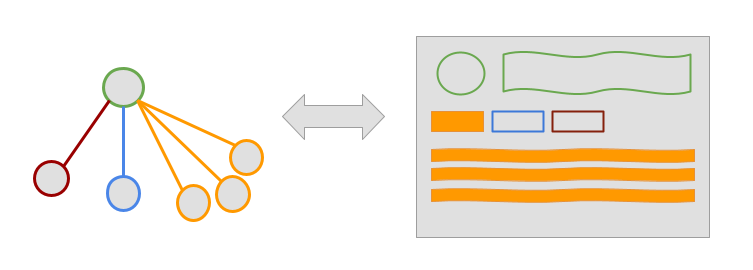
\includegraphics[width=1.0\linewidth]{Imagens/chap04/perfil-isomorfismo.png}
    \caption{Um \textcolor{green}{\textbf{nó X}} está relacionado à \textcolor{purple}{\textbf{um nó de rótulo Y}}, \textcolor{blue}{\textbf{um de rótulo W}}, e possui relação com \textcolor{orange}{\textbf{três nós de rótulos Z}} no grafo armazenado no banco de dados.}
    \label{fig:isomorphism}
\end{figure}


Temos então as propriedades do nó dono do perfil na parte superior da tela, e diferentes abas (uma para cada tipo de relação que o nó dono possui) na parte inferior, sendo que dentro de cada aba, uma lista de elementos com os nós vizinhos através daquele tipo de relação, com hiperlinks para páginas de perfis de seus vizinhos. Assim conseguimos andar pelo grafo através dos nós e relações, e em cada parada temos ações específicas como edição, criação ou conexão de nós.

Porém para o usuário começar esta navegação, ele precisa primeiro determinar o nó inicial. Essa é a função da chamada página de Lista, que como o nome sugere lista de maneira paginada e com funções de pesquisa os nós de algum rótulo específico, numa lista de elementos similar à uma aba dentro de um perfil. Permitindo agir sobre esses nós, ou entrar na página de perfil de um deles, começando a navegação pelos perfis.

A vantagem dessa modelagem é que conseguimos perceber que toda página de perfil (e de lista) segue a mesma regra, logo o código referente à sua implementação pode ser reutilizado. Ná prática a aplicação consiste em apenas uma página de perfil, e uma página de lista (além da página de login/autenticação), e mapas que definem as especificidades de cada caso, facilitando sua manutenção e minimizando o tamanho do seu código, consequentemente minimizando também bugs em produção.

\section{Arquitetura da Aplicação Cliente}
Building Blocks of a Web Application

There are a few things you need to consider when building modern applications. Such as:

    User Interface - how users will consume and interact with your application.
    Routing - how users navigate between different parts of your application.
    Data Fetching - where your data lives and how to get it.
    Rendering - when and where you render static or dynamic content.
    Integrations - what third-party services you use (CMS, auth, payments, etc) and how you connect to them.
    Infrastructure - where you deploy, store, and run your application code (Serverless, CDN, Edge, etc).
    Performance - how to optimize your application for end-users.
    Scalability - how your application adapts as your team, data, and traffic grow.
    Developer Experience - your team’s experience building and maintaining your application.
\subsection{Ações}

\section{Arquitetura do Servidor com endpoint GraphQL}

O frontend, entretando, não se comunica diretamente com o banco de dados, a interface se comunica com uma camada intermediária através de requisições em GraphQL, e esta camada intermediária gera a Cypher resultante que então é executada no banco de dados. Nesta seção descreveremos como funciona e a arquitetura escolhida para esta camada intermediária, o servidor que disponibiliza a endpoint em Graphql.

 \begin{figure}[H]

\begin{tikzpicture}[font=\small,thick]
 
% Start block
\node[draw,
    rounded rectangle,
    minimum width=2.5cm,
    minimum height=1cm] (block1) { Interface do ``Admins'' };
 
% Voltage and Current Measurement
\node[draw,
    below=0.8cm of block1,
    minimum width=2.5cm,
    minimum height=1cm
] (block2) { Servidor (Node.js) com endpoint GraphQL };
 
% Power and voltage variation
\node[draw,
    below=0.8cm of block2,
    minimum width=2.5cm,
    minimum height=1cm
] (block3) { Banco de Dados (Neo4j) };

\draw (block1) |- (block2);
\draw (block2) |- (block3);

\end{tikzpicture}
\caption{Fluxograma de comunicação entre partes do sistema }
\label{chap3:fluxograma}
\end{figure}

\subsection{Definições dos Tipos}

Uma das principais partes no servidor é a definição de cada tipo existente no banco de dados. Equivalente à definição das tabelas e campos num banco de dados SQL, é nessa etapa que modelamos os dados do domínio e definimos cada tipo de entidade que vai ter seu perfil, e pode ser interagida com a interface Admins.
Como se tratam de muitos tipos diferentes que interagem entre si, para fim de organização separamos eles em diferentes arquivos, cada um com seu escopo.

Cada arquivo possui os tipos referentes ao seu escopo, com suas propriedades e tipos das propriedades, suas relações e tipos dos nós que são relacionados, além de definir quais são as Queries e Mutations existentes na API GraphQL além das geradas automaticamente. Também nesses arquivos que definimos tipos não nativos, como ENUMs específicos do escopo. Os tipos vão definir quais são as Labels existentes no banco de dados.


\begin{lstlisting}
"""
Battles types
"""
type Battle implements Context @node(labels: ["Battle", "Context"]) {
	id: ID @id
	oldId: Int
	name: String
	type: ContextType
	status: ContextStatus
	createdAt: DateTime! @timestamp(operations: [CREATE])
	updatedAt: DateTime! @timestamp(operations: [CREATE, UPDATE])
	assignedContext: [AssignedContext!]!
		@relationship(type: "OF_CONTEXT", direction: IN)
	studentAnswers: [StudentAnswer]
		@cypher(
			statement: """
			MATCH (this)<-[:OF_CONTEXT]-(:AssignedContext)<-[:OF_ASSIGNED_CONTEXT]-(sa:StudentAnswer) return distinct sa
			"""
		)
	topic: Topic @relationship(type: "SELECTED_IN_BATTLE", direction: OUT)
	task: Task @relationship(type: "BATTLE_IN_TASK_CONTEXT", direction: OUT)
	fromOrigin: BattleOrigin #TODO: Improve the property
	students: [AssignedContext]
		@cypher(
			statement: """
			MATCH (this)<-[:OF_CONTEXT]-(ac:AssignedContext)-[:ASSIGNED_TO]->(s:Student) return distinct ac
			"""
		)
	startsAt: DateTime
	endsAt: DateTime
	knowledgeArea: KnowledgeArea
		@relationship(type: "IN_KNOWLEDGE_AREA", direction: OUT)
}

enum StudentBattleStatus {
	NotStarted
	InProgress
	Finished
	Refused
}

type Query {
	botQuestionAnswerFraction(
		studentProgressInPlanet: Float
		questionDifficulty: Float
	): Float
}

type Mutation {
	mergeStudentsBattle(
		studentsIds: [ID!]
		battleId: ID!
		type: ContextType
	): [ID]
	setBattleResult(battleId: ID!): String
	deleteBattle(battleId: ID!): ID
	setChampionshipBattleResults(championshipId: ID!): String
}
\end{lstlisting}

\subsection{Mesclador de Definições de Tipos}
A biblioteca Neo4j/GraphQL espera apenas um arquivo de definição de tipos, então precisamos juntar todos eles utilizando expressões regulares e os padrões de cada arquivo de definição de tipo.
\begin{lstlisting}
const fs = require("fs");
const path = require("path");

let typeDefs = "";
let mutations = "";
let queries = "";
let subscriptions = "";
const dirname = path.join(__dirname, "./types/");

export const mergeTypeDefs = () => {
	const filenames = fs.readdirSync(dirname);

	filenames.forEach((filename) => {
		let content = fs.readFileSync(dirname + filename, "utf-8");

		concatMutations(content);
		concatQueries(content);
		concatSubscriptions(content);

		content = removeMutationsQueriesAndSubscriptions(content);
		typeDefs += content;
	});

	typeDefs += mergeMutationsQueriesAndSubscriptions(typeDefs);

	return typeDefs;
};

const concatMutations = (typeDef) => {
	const re = /(?<=Mutation\s*\{)(.*?[\s\S]*?)(?=\n\}\n|\r\n\}\r\n)/g;
	const mutationsInTypeDef = typeDef.match(re);

	if (mutationsInTypeDef && mutationsInTypeDef.length > 0) {
		mutations = mutations.concat(...mutationsInTypeDef);
	}
};

const concatQueries = (typeDef) => {
	const re = /(?<=Query\s*\{)(.*?[\s\S]*?)(?=\n\}\n|\r\n\}\r\n)/g;
	const queriesInTypeDef = typeDef.match(re);

	if (queriesInTypeDef && queriesInTypeDef.length > 0) {
		queries = queries.concat(...queriesInTypeDef);
	}
};

const concatSubscriptions = (typeDef) => {
	const re = /(?<=Subscription\s*\{)(.*?[\s\S]*?)(?=\n\}\n|\n\}\n|\r\n\}\r\n)/g;
	const subscriptionsInTypeDef = typeDef.match(re);

	if (subscriptionsInTypeDef && subscriptionsInTypeDef.length > 0) {
		subscriptions = subscriptions.concat(...subscriptionsInTypeDef);
	}
};

const removeMutationsQueriesAndSubscriptions = (typeDef) => {
	const reMutations = /type\s*Mutation\s*\{(.*?[\s\S]*?)(\n\}\n|\r\n\}\r\n)/g;
	const reQueries = /type\s*Query\s*\{(.*?[\s\S]*?)(\n\}\n|\r\n\}\r\n)/g;
	const reSubscriptions = /type\s*Subscription\s*\{(.*?[\s\S]*?)(\n\}\n|\r\n\}\r\n)/g;

	let newTypeDef = typeDef.replaceAll(reMutations, "");
	newTypeDef = newTypeDef.replaceAll(reQueries, "");
	newTypeDef = newTypeDef.replaceAll(reSubscriptions, "");
	return newTypeDef;
};

const mergeMutationsQueriesAndSubscriptions = (typeDef) => {
	if (mutations.length > 0) {
		typeDef += `\r\n\r\ntype Mutation {\r\n${mutations}\r\n}`;
	}
	if (queries.length > 0) {
		typeDef += `\r\n\r\ntype Query {\r\n${queries}\r\n}`;
	}
	if (subscriptions.length > 0) {
		typeDef += `\r\n\r\ntype Subscription {\r\n${subscriptions}\r\n}`;
	}

	return typeDef;
};
\end{lstlisting}


\subsection{Geração do Schema e Escutando requisições}

No arquivo principal do servidor, o index.js, instanciamos o Express e configuramos suas conexões e middlewares. Utilizamos as bibliotecas padrões do driver Neo4j para conectar ao banco, autenticando com usuário e senha. Então importamos os nossos resolvers e definições de tipos, e configuramos os plugins utilizados, como o Neo4jGraphQLAuthJWTPlugin, que permite a autenticação das requisições através de uma JWToken no campo de "Authorization" no header de cada requisição GraphQL. Com tais informações geramos o Schema.

\begin{lstlisting}
async function initializeNeo4jGraphQL() {
	const neo4jGraphQL = new Neo4jGraphQL({
		driver,
		typeDefs: gql`
			${typeDefs}
		`,
		resolvers,
		plugins: {
			auth: new Neo4jGraphQLAuthJWTPlugin({
				secret: process.env.JWT_SECRET,
				algorithms: ["HS256"],
				credentialsRequired: false,
			}),
			config: {
				enableDebug: process.env.NODE_APP_ENV === "staging",
			},
		},
	});
	return await neo4jGraphQL.getSchema();
}
\end{lstlisting}

O Schema então é passado para o Apollo Server, e é dado seu start. O Express então sobe esse servidor nas portas definidas e fica escutando as requisições.